\documentclass[spanish]{article}
\usepackage[a4paper, left=1in, right=1in, top=1in, bottom=1in]{geometry}
                                % for page size and margin settings
\usepackage{graphicx}		    % for insert images
\usepackage[es-tabla]{babel} 	% for spanish titles
\usepackage[a4paper, left=1in, right=1in, top=1in, bottom=1in]{geometry} 
								% for page size and margin settings
\usepackage{mathtools}          % for greek math symbol formatting
\usepackage{enumitem}           % for control of 'enumerate' numbering
\usepackage{listings}           % for control of 'itemize' spacing
\usepackage{indentfirst}		% package to make first paragraph always indented
\usepackage{hyperref}           % page numbers and '\ref's become clickable
\usepackage{bm}					% for bold maths
\usepackage{setspace}			% for setting interline spacing
\usepackage{amsmath}			% for matrices
\usepackage{tikz} 				% for graphs
\usepackage{multirow}			% for tables
\usepackage{float}				% to manually select placement of tables
\usepackage{autobreak}          % to automatically fit equations to page width

\usetikzlibrary{babel}		    % for draw arrows in tikz using babel spanish
\renewcommand{\baselinestretch}{1.5}
\bibliographystyle{ieeetr}
\numberwithin{figure}{subsection}
\numberwithin{equation}{subsection}
\numberwithin{table}{subsection}

% TITLE VARIABLES 

\def\thesistitle{Incorporación de covariables que varían en el tiempo a un modelo mixto}
\def\thesisauthorfirst{\textbf{Esteban Cometto}}
\def\thesissupervisorfirst{Noelia Castellana}
\def\thesissupervisorsecond{Cecilia Rapelli}
\def\thesisdate{\today}

%% OTHER USEFUL VARIABLES 

\def\npatients{560}
\def\fullcovname{adherencia al tratamiento farmacológico}
\def\covname{\textit{adherencia}}
\def\cvt{covariable que varía en el tiempo}
\def\xseqj{$X_{i1}, ..., X_{ij}$}
\def\xseqn{$X_{i1}, ..., X_{in}$}
\def\xseqjminus{$X_{i1}, ..., X_{ij-1}$}
\def\yseqj{$Y_{i1}, ..., Y_{ij}$}
\def\yseqn{$Y_{i1}, ..., Y_{in}$}
\def\yseqjminus{$Y_{i1}, ..., Y_{ij-1}$}

%% FOR PDF METADATA
\title{\thesistitle}
\author{\thesisauthorfirst\space\thesisauthorsecond}
\date{\thesisdate}

\begin{document}

\begin{titlepage}
    \newcommand{\HRule}{\rule{\linewidth}{0.5mm}}
	\center
	\textsc{\Large Universidad Nacional de Rosario}\\[.7cm]
	
\includegraphics[width=25mm]{img/fceye-unr.png}\\[.5cm]
	\textsc{Facultad de Ciencias Económicas y Estadística}\\[0.5cm]
	\textsc{Anteproyecto de Tesina}
	
	\HRule \\[0.4cm]
	{ \huge \bfseries \thesistitle}\\[0.1cm]
	\HRule \\[.5cm]
	
	\begin{minipage}{0.6\textwidth}
	\large
	\textit{Autor:}	\thesisauthorfirst
	\end{minipage}
	\\[.6cm]
	\begin{minipage}{0.6\textwidth}
	\textit{Directora:} 	\thesissupervisorfirst \\[.2cm]
	\textit{Codirectora:} 	\thesissupervisorsecond
	\end{minipage}
	\\[4cm]
	\vfill
	{\large \thesisdate}\\
	\clearpage
\end{titlepage}

\newpage
\tableofcontents

\newpage
\section{Introducción}

Los datos longitudinales están conformados por mediciones repetidas sobre una
unidad, las cuales pueden surgir por ser medidas en diferentes momentos o
condiciones. Su principal objetivo es estudiar los cambios en el tiempo y los
factores que influencian el cambio. 

Los modelos mixtos permiten ajustar datos con estas características, donde la
respuesta se modela por una parte sistemática que está compuesta por una
combinación de características poblacionales que son compartidas por todas las
unidades (efectos fijos), y una parte aleatoria que está constituida por efectos
específicos de cada unidad (efectos aleatorios) y por el error aleatorio, las
cuales reflejan las múltiples fuentes de heterogeneidad y correlación entre y
dentro de las unidades.

En estos modelos pueden incorporarse covariables. Las mismas se pueden
clasificar en 2 categorías: covariables no variables en el tiempo (CNVT) y
covariables variables en el tiempo (CVT). La naturaleza diferente de estas
covariables conduce a considerar distintos enfoques para cada una de ellas en el
análisis.

Las CNVT son variables independientes que no tienen variación intra-unidad, es
decir que el valor de la covariable no cambia para una unidad determinada en
el estudio longitudinal. Este tipo de covariables se pueden utilizar para
realizar comparaciones entre poblaciones y describir diferentes tendencias en el
tiempo.

Las CVT son variables independientes que contienen ambas variaciones, intra y
entre unidad, es decir que el valor de la covariable cambia para una unidad
determinada a lo largo del tiempo y además puede cambiar para diferentes
unidades. Este tipo de covariables tienen los mismos usos que las CNVT, y además
permiten describir la relación dinámica entre la CVT y la respuesta. Sin
embargo, esta relación puede estar confundida por valores anteriores y/o
posteriores de la covariable y en consecuencia esto puede conducir a inferencias
engañosas sobre los parámetros del modelo. Esta tesina realiza una introducción
a la problemática de incorporar covariables que varían en el tiempo en modelos
mixtos para datos longitudinales, presentando diferentes definiciones de las
mismas y enfoques metodológicos.

Estos conceptos se aplican a un conjunto de datos que surge del programa de
atención y control de pacientes hipertensos de Fundación ECLA llevado a cabo en
Rosario durante el período 2014-2019. Este estudio observacional realizó un
seguimiento de un grupo de pacientes hipertensos registrando en cada visita el
tratamiento farmacológico dado al paciente, los valores de la tensión arterial
sistólica (TAS) y la adherencia a dicho tratamiento entre otras características.
Uno de los objetivos que persiguió este estudio fue evaluar si la adherencia al
tratamiento influye en los valores de la TAS a lo largo del seguimiento. Como la
variable adherencia es una CVT, se presentarán diferentes enfoques para
incluirla en un modelo longitudinal mixto que pueda explicar el cambio en la
tensión arterial sistólica media a lo largo del tiempo.

\newpage
\section{Objetivos}

\subsection{Objetivo Principal}

Presentar diferentes propuestas metodológicas para la incorporación de
covariables que varían con el tiempo en modelos mixtos para datos
longitudinales.

\subsection{Objetivos Específicos}

\begin{itemize}
	\item Definir los tipos de covariables existentes.
	\item Describir propuestas de incorporación de covariables que varían en el
	tiempo en los modelos mixtos.
	\item Aplicar los conceptos vistos al programa de
	atención y control de pacientes hipertensos de Fundación ECLA.
\end{itemize}

\newpage
\section{Datos Longitudinales}

Los datos longitudinales están conformados por mediciones repetidas de una misma
variable realizadas a la misma unidad en diferentes momentos o condiciones
experimentales.

Dado que las mediciones repetidas son obtenidas de la misma unidad, los datos
longitudinales están agrupados. Las observaciones dentro de un mismo
agrupamiento generalmente están correlacionadas positivamente. Por lo tanto, los
supuestos usuales de independencia y homogeneidad de variancias no son válidos

Existen tres fuentes potenciales de variabilidad que influyen sobre la
correlación entre medidas repetidas:

\begin{itemize}
	\item \textit{Heterogeneidad entre las unidades:} Refleja la propensión
	natural de las unidades a responder. Las unidades tienen diferentes
	reacciones frente a los mismos estímulos.
	\item \textit{Variación biológica intra-unidad:} Se espera que la secuencia
	de medidas repetidas de una unidad tenga un comportamiento determinado, que
	produce que las mediciones más cercanas sean más parecidas entre sí que las
	más alejadas.
	\item \textit{Error de medición:} Errores aleatorios asociados al proceso de
	medición.
\end{itemize}

Estas tres fuentes de variación pueden clasificarse en \textit{``variabilidad
entre unidades''} (heterogeneidad entre unidades) y \textit{``variabilidad
intra unidades''} (variación biológica intra-unidad y error de medición)

Dado que estas fuentes de variabilidad introducen correlación entre las
mediciones repetidas, no se pueden utilizar las técnicas habituales, ya que
llevarían a inferencias incorrectas sobre los parámetros del modelo.

Con el fin de simplificar la notación, se asumirá que los tiempos de medición
son los mismos para todas las unidades y que no hay datos faltantes.

Sean $Y_{ij}$ el valor de la variable respuesta y $X_{ij}$ las covariables,
medidas sobre la unidad $i$ en la ocasión $j$, se obtiene una muestra de $N$
unidades cada una con $n$ mediciones repetidas de la variable en estudio,
observadas en los tiempos $t_1, t_2, ..., t_n$, siendo entonces el número total
de observaciones $N^*=Nn$, con $i=1, ..., N; j=1, ..., n$.

Se asume que $Y_{ij}$ y $X_{ij}$ son simultáneamente medidas. Esto quiere decir
que en un análisis de corte transversal, $Y_{ij}$ y $X_{ij}$ se correlacionan
directamente. Sin embargo, para un análisis longitudinal se debe asumir que
existe un orden pre-establecido:
$(X_{i1}, Y_{i1}), (X_{i2}, Y_{i2}), ..., (X_{in}, Y_{in})$

\section{Covariables en datos longitudinales}

En los estudios longitudinales, las variables independientes pueden ser
clasificadas en dos categorías: CNVT y CVT. La diferencia entre
ellas puede conducir a diferentes enfoques de análisis así como también a
diferentes conclusiones.

Tanto las CNVT como las CVT se pueden utilizar para realizar comparaciones entre
poblaciones y describir diferentes tendencias a lo largo del tiempo. Sin
embargo, sólo las CVT permiten describir una relación dinámica entre la
covariable y la variable respuesta.

\subsection{Covariables fijas en el tiempo}

Las CNVT son variables independientes que no presentan variación intra-unidad,
es decir, los valores de estas covariables no cambian a lo largo del estudio
para una unidad en particular.

Éstas covariables pueden ser fijas por naturaleza (por ejemplo, el sexo
biológico de una persona o el grupo de tratamiento) o pueden ser covariables
basales (es decir, medidas al inicio del estudio). Las covariables basales son
fijas por definición pero pueden ser variables en el tiempo por naturaleza, por
ejemplo, la edad varia en el tiempo pero la edad basal es fija.

\subsection{Covariables variables en el tiempo}

Las CVT son variables independientes que incluyen tanto la variación
intra-unidad como la variación entre-unidad. Esto significa que, para una unidad
en particular, el valor de la covariable cambia a través del tiempo y puede
cambiar también entre diferentes unidades. Por ejemplo, el valor del colesterol
o la condición de fumador (si/no).

A continuación se describen diferentes tipos de CVT.

\subsubsection{Covariables estocásticas y no estocásticas}

Las CVT pueden clasificarse en estocásticas y no estocásticas. Las CVT no
estocásticas son covariables que varían sistemáticamente a través del tiempo
pero son fijas por diseño del estudio o bien su valor puede predecirse. En
cambio, las CVT estocásticas son covariables que varían aleatoriamente a través
del tiempo, es decir, los valores en cualquier ocasión no pueden ser estimados
ya que son gobernados por un mecanismo aleatorio. Ejemplos de las primeras son:
tiempo desde la visita basal o edad. Ejemplos de las segundas son: valor del
colesterol, ingesta de alcohol (si/no), ingesta de grasas, etc.

\subsubsection{Covariables exógenas y endógenas}
\label{seccion_de_exogeneidad}

Otra clasificación de las CVT es en exógenas y endógenas.

\paragraph{Covariables exógenas} \mbox{} \\

Una CVT se define como exógena, respecto a la variable respuesta, si el valor de
la covariable en un determinado momento es condicionalmente independiente de
todos los valores precedentes de la variable respuesta. Formalmente, para la
unidad $i$ en la ocasión $j$:  

\begin{equation}
	\label{exogeneidad}
	f(X_{ij}|X_{i1}, ..., X_{ij-1}, Y_{i1}, ..., Y_{ij}) =
	f(X_{ij}|X_{i1}, ..., X_{ij-1})
\end{equation}

Y en consecuencia:

\begin{equation}
	\label{exogeneidad debil}
	E(\bm{Y_i}|\bm{X_i}) = E(\bm{Y_i}|X_{i1}, ..., X_{in}) = E(\bm{Y_i}|X_{i1}, ..., X_{ij})
\end{equation}

Esta definición implica que la respuesta en cualquier momento puede depender de
los valores previos de la variable respuesta y de la CVT, pero será
independiente de todos los demás valores de la covariable. Por ejemplo, en un
estudio longitudinal en donde se evalúa si el nivel de polución en el aire está
asociado a la función pulmonar, es de esperar que el nivel de polución del aire
en una determinada ocasión dependa de los niveles observados previamente, pero
no se espera que dependa de los niveles de la función pulmonar observados
previamente en el sujeto.

Es posible examinar empíricamente la suposición de que una CVT es exógena al
considerar modelos de regresión para la dependencia de $X_{ij}$ en
$Y_{i1}, ..., Y_{ij-1}$ (o en alguna función conocida de
$Y_{i1}, ..., Y_{ij-1}$) y $X_{i1}, ..., X_{ij-1}$ (o en alguna función conocida
de $X_{i1}, ..., X_{ij-1}$). La ausencia de cualquier relación entre $X_{ij}$ y
$Y_{i1}, ..., Y_{ij-1}$, dado el perfil de la covariable anterior
$X_{i1}, ..., X_{ij-1}$, proporciona soporte para la validez de la suposición de
que la CVT es exógena.

Cuando se puede asumir que las CVT son exógenas con respecto a la variable
respuesta, se puede dar una interpretación causal a los parámetros de regresión.

\paragraph{Covariables endógenas} \mbox{} \\

Una CVT que no es exógena se define como endógena. Una variable endógena es una
variable estocásticamente relacionada con otros factores medidos en el estudio.
Esta también puede definirse como una variable generada por un proceso
estocástico relacionado con el individuo en estudio. En otras palabras, las CVT
endógenas están asociadas con un efecto individual y, a menudo, pueden
explicarse por otras variables en el estudio. Cuando el proceso estocástico de
una CVT endógena puede ser (al menos parcialmente) explicado por la variable
respuesta, se dice que hay \textit{feedback} entre la respuesta y la CVT
endógena. Por ejemplo, cuando se evalúa si la cantidad de actividad física está
asociada al nivel de glicemia. El nivel de actividad física en un determinado
momento puede estar (o no) asociado a niveles previos y también puede estar
asociado a valores previos de glicemia (un paciente con valor de glicemia alto
en una visita puede decidir aumentar su nivel de actividad fística para ver si
este valor se reduce).

\section{Modelo lineal mixto}

Los modelos lineales mixtos se utilizan habitualmente para analizar los datos
longitudinales, debido a que permiten modelar las distintas fuentes de
variabilidad presentes en los mismos.

En estos modelos, la respuesta media se modela como una combinación de
características poblacionales que son comunes a todos los individuos (efectos
fijos) y efectos específicos de la unidad que son únicos de ella (efectos
aleatorios).

El modelo lineal mixto para la unidad $i$ se puede expresar en forma matricial
como:

\[
	\bm{Y}_i = \bm{X}_i\bm{\beta} + \bm{Z}_i\bm{b}_i + \bm{\varepsilon}_i;
	\quad i = 1, ..., N;
\]

Donde:

\begin{itemize}
	\item $\bm{Y}_i$: Vector de la variable respuesta de la i-ésima unidad, de
	dimensión $(n \times 1)$, siendo $\bm{Y}_i = (Y_{i1}, Y_{i2}, ... Y_{in})'$
	\item $\bm{X}_i$: Matriz de diseño de la i-ésima unidad, que caracteriza la
	parte sistemática de la respuesta, de dimensión $(n \times p)$
	\item $\bm{\beta}$: Vector de parámetros de dimensión $(p \times 1)$
	\item $\bm{Z}_i$: Matriz de diseño de la i-ésima unidad, que caracteriza la
	parte aleatoria de la respuesta, de dimensión $(n \times k)$
	\item $\bm{b}_i$: Vector de efectos aleatorios de la i-ésima unidad, de
	dimensión $(k \times 1)$
	\item $\bm{\varepsilon}_i$: Vector de errores aleatorios de la i-ésima unidad,
	de dimensión $(n \times 1)$
\end{itemize}

Se supone que $\bm{\varepsilon}_i$ y $\bm{b}_i$ son independientes.

\[ \bm{\varepsilon}_i \sim N_{n}(0, \bm{R}_i) \]
\[ \bm{b}_i \sim N_k(0, \bm{D}) \]

$\bm{D}$ y $\bm{R}_i$ son las matrices de variancias y covariancias de los
vectores $\bm{b}_i$ y $\bm{\varepsilon}_i$ respectivamente. A partir de este
modelo se obtiene:

\begin{itemize}
	\item $E(\bm{Y}_i/\bm{b}_i) = \bm{X}_i\bm{\beta} + \bm{Z}_i\bm{b}_i$ (media condicional o específica de
	la i-ésima unidad)
	\item $E(\bm{Y}_i) = \bm{X}_i\bm{\beta}$ (media marginal)
	\item $Cov(\bm{Y}_i/\bm{b}_i) = \bm{R}_i$ (variancia condicional)
	\item $Cov(\bm{Y}_i) = \bm{Z}_i \bm{D}_i \bm{Z}'_i + \bm{R}_i = \bm{\varSigma}_i$ (variancia marginal)
\end{itemize}

Generalmente, la matriz $\bm{D}$ adopta una estructura de covariancia
arbitraria, mientras que la matriz $\bm{R}_i$ adopta otra estructura que modela
apropiadamente la variabilidad intra individuo.

\subsection{Estimación de los parámetros del modelo}

Bajo el supuesto de que $\bm{\varepsilon}_i$ y $\bm{b}_i$ se distribuyen normalmente se
pueden usar métodos de estimación basados en la teoría de máxima verosimilitud,
cuya idea es asignar a los parámetros el valor más probable en base a los datos
que fueron observados. Se usarán para estimar los parámetros de la parte media
y los de las estructuras de covariancia los métodos de máxima verosimilitud
(ML) y máxima verosimilitud restringida (REML) respectivamente

\subsubsection{Método de máxima verosimilitud (ML)}

Bajo el supuesto de que $\bm{Y}_i \sim N_n(\bm{X}_i \bm{\beta},
\bm{\varSigma}_i)$ y las $\bm{Y}_i$
son independientes entre sí, se obtiene la siguiente función de
log-verosimilitud:

\begin{equation}
\label{ML}
	l = -\frac{1}{2} \sum_{i=1}^{N}n ln(2\pi) - \frac{1}{2}ln|\bm{\varSigma}_i| -
	\frac{1}{2} \sum_{i=1}^{N} [(\bm{Y}_i - \bm{X}_i\bm{\beta})'
	\bm{\varSigma}_i^{-1} (\bm{Y}_i - \bm{X}_i\bm{\beta})]
\end{equation}

Siendo $\bm{\varSigma}_i$ función del vector $\bm{\theta}$ que contiene los
parámetros de covariancia.

Los estimadores de $\bm{\beta}$ y $\bm{\theta}$ son los valores que maximizan
esta expresión. Cuando $\bm{\theta}$ es desconocido (lo que generalmente sucede)
se obtiene una ecuación no lineal, por lo que no se puede obtener una expresión
explícita de $\hat{\bm{\theta}}$. Para encontrar su solución se recurre a
métodos numéricos. El estimador del vector $\bm{\beta}$ resulta:

\[ \hat{\bm{\beta}} = (\sum_{i=1}^{N} \bm{X}_i'\hat{\bm{\varSigma}_i}^{-1}\bm{X}_i)^{-1}
\sum_{i=1}^{N} \bm{X}'_i\hat{\bm{\varSigma}_i}^{-1}\bm{Y}_i \]

El estimador $\hat{\bm{\beta}}$ resulta insesgado de $\bm{\beta}$. Cuando
$\bm{\theta}$ es desconocido no se puede calcular de manera exacta la matriz
de covariancias de $\hat{\bm{\beta}}$. Si el número de unidades es grande se
puede demostrar que asintóticamente (Fitzmaurice et al., 2004):

\[ \hat{\bm{\beta}} \sim N_p(\bm{\beta}, \bm{V}_{\bm{\beta}}) \quad donde \quad \bm{V}_{\bm{\beta}} =
(\sum_{i=1}^{N} \bm{X}'_i\hat{\bm{\varSigma}_i}^{-1}\bm{X}_i)^{-1} \]

\subsubsection{Método de máxima verosimilitud restringida (REML)}

El inconveniente que posee el método de ML es que los parámetros de covariancia
resultan sesgados. Es decir, a pesar de que $\bm{\hat{\beta}}$ es un estimador
insesgado de $\bm{\beta}$, no pasa lo mismo con $\bm{\hat{\theta}}$. Si el
tamaño de muestra es chico, los parámetros que representan las variancias van a
ser demasiado pequeños, dando así una visión muy optimista de la variabilidad de
las mediciones, es decir, se subestiman los parámetros de covariancia. El sesgo
se debe a que en la estimación ML de $\bm{\theta}$ no se tiene en cuenta que
$\bm{\beta}$ es estimado a partir de los datos.

Distintos autores proponen el método de REML para estimar los parámetros del
modelo. Este método es una modificación del método de máxima verosimilitud, en
el que la parte de los datos usada para estimar $\bm{\beta}$ está separada de
aquella usada para estimar los parámetros de $\bm{\varSigma}_i$. La función de
log-verosimilitud restringida que se propone es:

\begin{equation}
\label{REML}
	\bm{l}^* = -\frac{1}{2} \sum_{i=1}^{N}n ln(2\pi) - \frac{1}{2}ln|\bm{\varSigma}_i| -
	\frac{1}{2} \sum_{i=1}^{N} [(\bm{Y}_i - \bm{X}_i\bm{\beta})'
	\bm{\varSigma}_i^{-1} (\bm{Y}_i - \bm{X}_i\bm{\beta})] -
	- \frac{1}{2} ln |\sum_{i=1}^{N} \bm{X}'_i \hat{\bm{\varSigma}_i^{-1} \bm{X}_i}|
\end{equation}

Maximizando esta funcion con respecto a $\bm{\beta}$ y $\bm{\theta}$ se obtiene:

\[ \hat{\bm{\beta}} = (\sum_{i=1}^{N} \bm{X}'_i \hat{\bm{\varSigma}}_i^{-1} X_i)^{-1}
\sum_{i=1}^{N} \bm{X}'_i \hat{\bm{\varSigma}}_i^{-1} \bm{Y}_i\]

Donde $\hat{\bm{\varSigma}}_i$ es el estimador REML de ${\bm{\varSigma}_i}$

\subsubsection{Problemas con la estimación}

Pepe y Anderson (1994) mostraron que las ecuaciones \ref{ML} y \ref{REML} llegan
a cero solo si se cumple con el supuesto de independencia condicional:

\begin{equation}
\label{estimation_issue}
	E[\bm{Y}_{ij} | \bm{X}_{ij}] = E[\bm{Y}_{ij} | \bm{X}_{ij}, j = 1, ..., n]
\end{equation}

Con las CNVT, esta suposición se mantiene necesariamente ya que $X_{ij} =
X_{ik}$ para todas las ocasiones $k \neq j$. Con las CVT estocásticas, que se
fijan por diseño del estudio (por ejemplo, indicador de grupo de tratamiento en
una prueba cruzada), la suposición también se cumple ya que los valores de las
covariables en cualquier ocasión se determinan a priori por diseño del estudio y
de manera completamente no relacionado con la respuesta longitudinal. Sin
embargo, cuando una covariable es variable en el tiempo no estocástica, puede
que no necesariamente se mantenga.

En general, cuando (\ref{estimation_issue}) no se cumple, los valores
precedentes y/o posteriores de la CVT confunden la relación entre $Y_{ij}$ y
$X_{ij}$, esto puede llevar a estimaciones sesgadas de los parámetros del
modelo.

Frente a este escenario, Pepe y Anderson (1994) recomendaron plantear el modelo
longitudinal marginal y realizar las estimaciones mediante GEE (ecuaciones de
estimación generalizadas) con estructura de correlación independiente ya que
este es siempre consistente. La estructura de correlación independiente
generalmente tiene una alta eficiencia para la estimación de los coeficientes
asociados a CNVT. Sin embargo, para las CVT, Fitzmaurice (1995) muestra que esta
estructura puede resultar en una pérdida sustancial de eficiencia para la
estimación de los coeficientes asociados a las CVT y proporciona un ejemplo en
el que es sólo un 60\% eficiente en relación con la estructura de correlación
verdadera.

Por otro lado, Lai y Small (2007) definieron 3 tipos de CVT y luego Lalonde et.
al (2014) definieron un cuarto tipo de CVT. Además, propusieron utilizar el
``Método generalizado de los momento'' (GMM) (Hansen, 1982) en el cual se puede
incorporar información sobre la naturaleza de la CVT que se está analizando
según su tipo.

En conclusión, para poder utilizar una CVT en un modelo lineal mixto, esta debe
cumplir la condicion de exogeneidad. En el siguiente apartado se describen
diferentes formas en las que se puede incluir la CVT exógena al modelo lineal
mixto.

\newpage

%%%%%%%%%%%%%%%%%%%%%%%%%%%%%%%%%%%%%%%%%%%%%
% REESCRIBIR TODA ESTA SECCION (VER DIGGLE) %
%%%%%%%%%%%%%%%%%%%%%%%%%%%%%%%%%%%%%%%%%%%%%

\section{Formas de introducir una CVT al modelo}

Si al evaluar el tipo de la CVT de la manera vista en
\ref{seccion_de_exogeneidad} resulta ser exógena, se puede introducir en el
modelo mixto sin consideraciones adicionales. Esto se debe a que no habrá
problemas con la estimación de los parámetros, ya que se cumple el supuesto de
independencia condicional.

A continuación, se presentan distintas maneras de introducir la CVT exógena al
modelo mixto. De manera de ejemplo, se tomará un caso en el que la variable
respuesta $Y_{ij}$ y la CVT $X_{ij}$ son la tensión arterial y el IMC,
respectivamente, del paciente $i$ en la ocasión $j$.

\subsection{Convertirla en CNVT}

Una solución rápida al problema de las CVT, sea exógena o endógena, es
transformarla en una CNVT, esto se puede lograr resumiendo la información de la
misma mediante alguna función como el promedio de los valores de cada individuo
y dejarlo fijo a través del tiempo. También podria usarse su valor máximo,
mínimo o cualquier transformación que resulte de interés en el estudio. El
problema de este enfoque es que se pierde mucha información, dado que se usa una
covariable más simple que no refleja la relación dinámica entre la covariable y
la respuesta en el tiempo.

En el ejemplo mencionado anteriormente, se podría calcular el IMC promedio de
cada uno de los individuos y el modelo resultaría:

\[ Y_{ij} = \beta_0 + \beta_1 \overline{X}_i + \epsilon_{i} \]

El coeficiente $\beta_1$ se interpreta como el cambio en la tensión arterial por
cada cambio unitario en el IMC promedio del individuo.

\subsection{Covariable variable en el tiempo}

Dado que la CVT es exógena, se puede incorporar al modelo sin ninguna
transformación. El modelo resultante es,

\[ Y_{ij} = \beta_0 + \beta_1 X_{ij} + \epsilon_{i} \]

Como se mencionó anteriormente, las CVT contienen efecto intra-unidad y
entre-unidad, sin embargo el modelo mixto va a tener solo un coeficiente
$\beta_1$. Por lo tanto, el modelo mixto asume convergencia entre los efectos
intra-unidad y entre-unidad (es decir, que son equivalentes y ambos pueden ser
representados como un único efecto). Si bien el modelo es válido, para obtener
una interpretación clara del efecto de la CVT se necesita dividir su efecto en
dos coeficientes, como se explicará en la sección \ref{Dividiendo efecto
entre-unidad y efecto intra-unidad}

%%%% LESSA HOFFMAN PAGINA 345

\subsection{Covariable rezagada}

En algunas aplicaciones hay justificacion previa para considerar la covariable
en el rezago $k$ momentos antes de la medición de la respuesta. Por ejemplo, el
efecto del IMC sobre la tensión arterial probablemente no sea inmediato, por lo
que podría interesarnos su valor en la ocasión anterior ($k=1$). Lo más común es
que se desconozca el valor $k$ apropiado y se consideren varias opciones
diferentes. El modelo mixto se definiría de la siguiente manera:

\[ Y_{ij} = \beta_0 + \beta_{1k} X_{ij-k} + \epsilon_{i} \]

En este modelo, el coeficiente $\beta_{1k}$ depende explícitamente de la
elección del rezago $k$.

\subsection{Funcion de las covariables rezagadas}

Una alternativa cuando se quiere utilizar la información de las covariables
rezagadas es resumir a través de una función la información de éstas en una sola
covariable. Un ejemplo puede ser el valor promedio o acumulado hasta la ocasión
actual. Sin embargo, la elección de está funcion dependerá del tipo de problema
a analizar. Cabe destacar que, al igual que con toda medida resumen, al usar
este tipo de covariables se pierde parte de la información. En el ejemplo
mencionado, podría ser de interés calcular el IMC promedio hasta la ocasión $j$,
resultando el modelo:

\[ Y_{ij} = \beta_0 + \beta_1 \overline{X}_{ij} + \epsilon_{i} \]

Donde $\overline{X}_{ij}$ es el IMC promedio calculado hasta la ocasión $j$

\subsection{Dividiendo efecto entre-unidad y efecto intra-unidad}
\label{Dividiendo efecto entre-unidad y efecto intra-unidad}

Otra forma de incorporar la CVT es dividiendo el efecto en dos componentes que
reflejen la variación intra-unidad y la variación entre-unidad. Entonces, el
coeficiente del modelo que representa a la covariable se puede descomponer en
dos:

\[ Y_{ij} = \beta_0 + \beta_W (X_{ij} - \overline{X}_i) + \beta_B \overline{X}_i + \epsilon_{i} \]

Donde, $\overline{X}_i$ representa el promedio de todos los valores observados
en el tiempo de la CVT para la unidad $i$, $\beta_W$ representa el cambio
esperado en la media de la variable respuesta asociado con cambios de la CVT
dentro de la unidad y $\beta_B$ representa el cambio esperado en la media de
la variable respuesta asociado con cambios de la CVT entre unidades

En el ejemplo del IMC y la tensión arterial, $\beta_W$ se interpreta como el
cambio en la tensión arterial por cada diferencia de una unidad en el IMC de la
ocasión $j$ comparado con el IMC promedio de la persona, manteniendo constante
el IMC de las ocasiones restantes. Por otro lado, $\beta_B$ se interpreta como
el cambio en la tensión arterial por cada cambio de una unidad en el IMC
promedio de la unidad, controlando por el valor del IMC de la ocasión $j$.

Estos dos efectos permiten medir entonces si la tensión arterial aumenta cuando
una persona tiene un IMC mayor que el promedio de la población, y también
permiten medir el cambio en la tensión arterial si dicha persona tiene IMC mayor
que su promedio habitual.

\newpage

\section{Aplicación}

Se cuenta con un programa de atención y control de pacientes hipertensos
iniciado en el año 2014 en Rosario que realiza un seguimiento exhaustivo de
\npatients{} pacientes de entre 30 y 86 años, con una edad media de 58.84 y
desvío estándar de 9.87 años, de los cuales un 49.28\% son hombres. Las visitas
se realizaron una vez por mes durante 7 meses desde asignado el tratamiento y en
cada una de ellas se registró si la persona estaba adhiriendo correctamente al
tratamiento y el valor de la tensión arterial sistólica (TAS) (M=134.10,
DS=16.07). Es decir, el seguimiento comenzó a medirse luego de un mes de que los
pacientes empezaron el tratamiento.

A fines de centrarse en la CVT se dejaron de lado algunas covariables fijas
derivadas de estudios de laboratorio, manteniendo solo algunas covariables
sociodemográficas de interés para lograr una estabilidad entre modelos
interpretables pero no demasiado complejos, sin perder el objetivo principal de
este informe.

\subsection{Análisis descriptivo}

En esta sección se presentaran diversos gráficos con el fin de describir la
población en estudio.

En la figura \ref{TAS_vs_tpo} se puede observar que en general la TAS se
mantiene constante (o con una muy leve pendiente decreciente) a través del
tiempo. Esto a simple vista podría resultar desalentador, dado que el propósito
del tratamiento es disminuir la TAS a niveles más saludables. Sin embargo, como
se mencionó anteriormente, los pacientes no adhirieron al 100\% el tratamiento,
este efecto es el que estudiaremos más adelante. Cabe destacar que las
mediciones de los pacientes son equiespaciadas en el tiempo, las desviaciones
del eje en el tiempo se deben a una técnica llamada ``jitter'' que nos permite
mover levemente los puntos en el eje x para poder observar mejor la densidad de
los mismos. 

\begin{figure}[H]
	\centering
	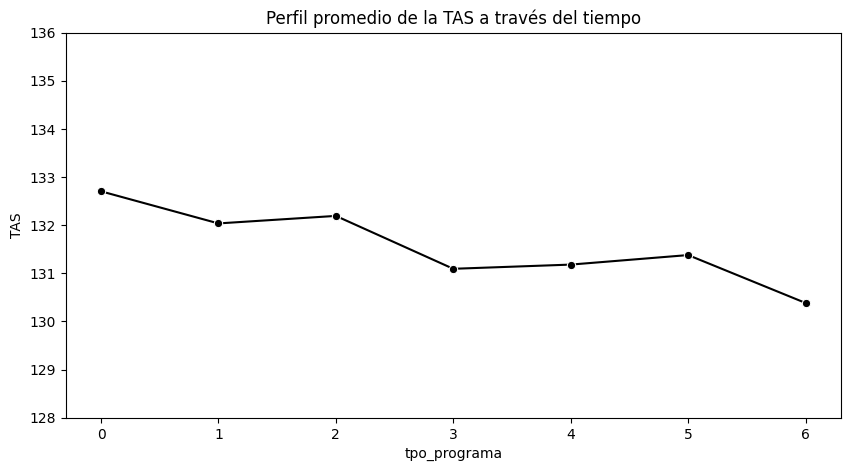
\includegraphics[scale=0.5]{img/TAS_vs_tpo.png}
	\caption{TAS de cada paciente en cada tiempo}
	\label{TAS_vs_tpo}
\end{figure}

En la figura \ref{spaghetti} se pueden observar las trayectorias individuales
de 15 pacientes seleccionados al azar, las pendientes son muy similares entre
sí, sin embargo hay variación en la ordenada al origen.

\begin{figure}[H]
	\centering
	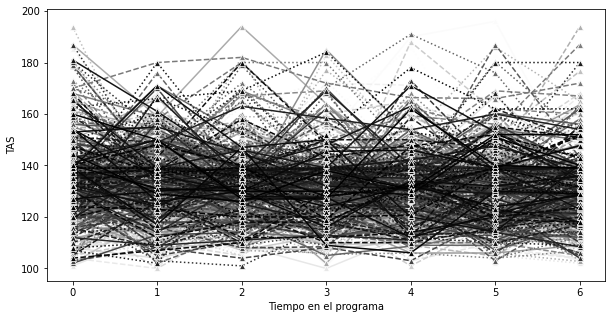
\includegraphics[scale=0.5]{img/spaghetti_plot.png}
	\caption{TAS a través del tiempo de 15 pacientes al azar}
	\label{spaghetti}
\end{figure}

Otro gráfico que resulta de interés es observar la evolución de la TAS a través
del tiempo pero sobre cada grupo de las covariables fijas, el resultado se
expresa en la figura \ref{TAS_with_covs}. Para las variables continuas, se
utilizó como punto de corte para segmentar en grupos la mediana de sus valores.
Podemos observar que en general la TAS disminuye, ya sea en mayor o menor
medida, a los largo del tiempo. Analizando las covariables una por una, el IMC
parece no tener un efecto significativo, dado que, aunque los pacientes con
menor IMC presentan menor TAS, los promedios en cada tiempo caen dentro de los
intervalos de confianza de ambos grupos. En cuanto a la edad y el sexo, no
parece haber una diferencia significativa en las pendientes pero si parece haber
una leve diferencia en las ordenadas al origen, presentando menor TAS los
pacientes más jóvenes y de sexo femenino. Por último, los pacientes con
antecedentes de diabetes parecen tener una TAS mayor en un comienzo con una
pendiente negativa a través del tiempo, mientras que los pacientes que no tienen
antecedentes de diabetes comienzan con una TAS mas inferior manteniendola más
constante.

\begin{figure}[H]
	\centering
	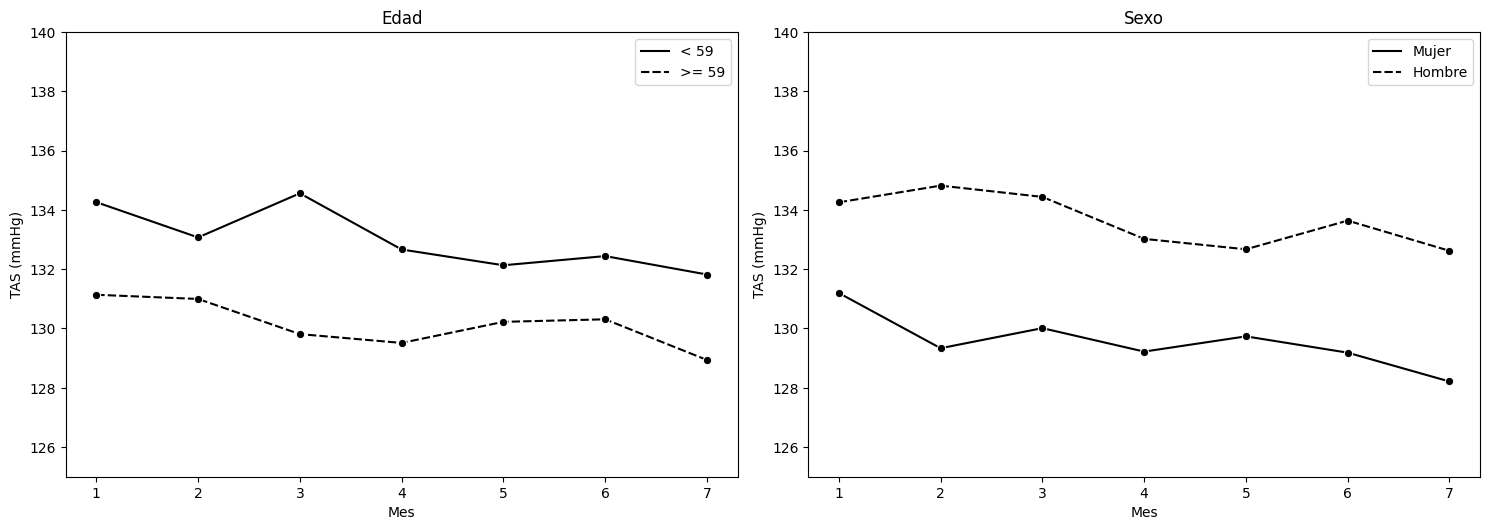
\includegraphics[scale=0.4]{img/TAS_vs_tpo_with_covs.png}
	\caption{TAS a través del tiempo según grupos de covariables}
	\label{TAS_with_covs}
\end{figure}

Por último, la figura \ref{TAS_with_adh} refleja el efecto de la adherencia al
tratamiento sobre la TAS. Para mantener perfiles no variables en el tiempo, se
usa la adherencia total al tratamiento y al igual que antes se divide en base a
su mediana, teniendo por un lado los pacientes que adhieren correctamente a más
del 86\% del tratamiento (al menos 6 de las 7 ocasiones) y por el otro a los
pacientes que adhieren correctamente menos del 86\% del tratamiento (hasta 5 de
las 7 ocasiones). Aqui se puede observar que los pacientes que adhieren
correctamente al tratamiento parecen tener una pendiente negativa en la TAS a
través del tiempo, mientras que los pacientes que no adhieren correctamente
mantienen la TAS más constante.

\begin{figure}[H]
	\centering
	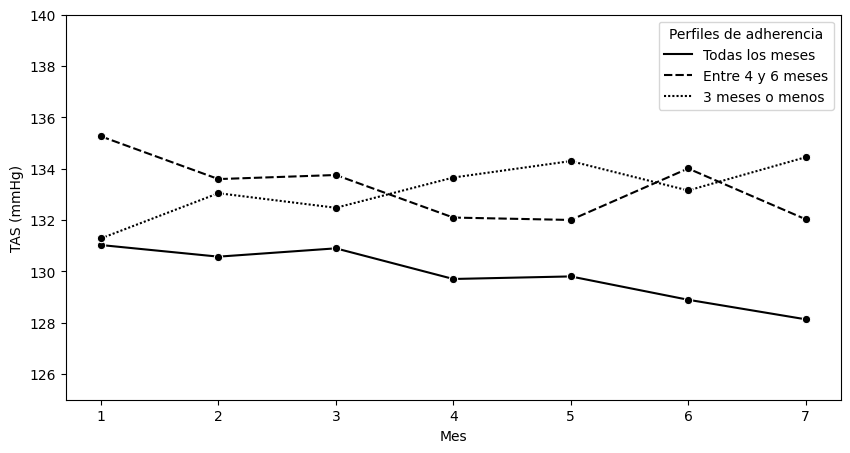
\includegraphics[scale=0.5]{img/TAS_vs_tpo_with_adherencia.png}
	\caption{TAS a través del tiempo según adherencia al tratamiento}
	\label{TAS_with_adh}
\end{figure}

\subsection{Modelo propuesto}

\subsubsection{Modelo propuesto para la media}

El modelo propuesto \ref{modelo_simple} es un modelo simple sin interacciones
entre covariables, a pesar de que algunas de ellas podían resultar
significativas, con fines de facilitar las interpretaciones de las distintas
maneras de incluir la CVT al modelo.

\begin{multline}
	\label{modelo_simple}
	\hat{y}_{ij} = 121.311\ +\ b_{0i}\ +\ 3.911\ sexo_i\ +\ 0.158\ edad_i\
	-\ 0.332\ mes_j\ +\ b_{1i}*mes_j\
\end{multline}

\subsubsection{Modelo propuesto para la covariancia}

En la figura \ref{semivariogram} puede notarse que la mayor parte de la
variabilidad total está compuesta por el error de medición dado que la curva no
inicia en el cero. Al no haber una pendiente muy pronunciada, la correlación
serial también puede considerarse pequeña. Por último, como la curva no llega a
la variancia total, esto nos indica que debe explicarse la variancia entre
individuos agregando una ordenada aleatoria (ver Anexo
\ref{eleccion_efectos_aleatorios}).

%%%%%%%%%%%%%%%%%%%%%%%%%%%%
% AGREGAR PROCESO AL ANEXO %
%%%%%%%%%%%%%%%%%%%%%%%%%%%%

\begin{figure}[H]
	\centering
	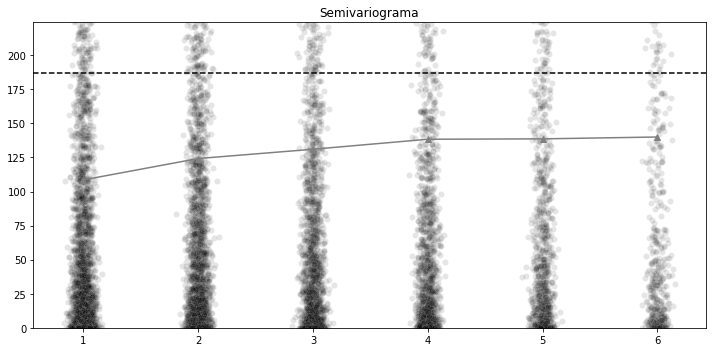
\includegraphics[scale=0.4]{img/semivariogram.png}
	\caption{Semivariograma}
	\label{semivariogram}
\end{figure}

Además, se realizaron tests de hipótesis para probar la significación de los
efectos aleatorios para la ordenada y la pendiente, resultando ambos
significativos. Por lo que la estructura de covariancia elegida para el modelos
es una estructura independiente con ordenada y pendiente aleatoria.

Los resultados obtenidos con el modelo propuesto pueden observarse en la tabla
\ref{modelo_1}.

\begin{table}[H]
	\centering
	\caption{Modelo 1: Modelo propuesto sin CVT}
	\label{modelo_1}
	\begin{tabular}{*{5}{|c}|}
		\hline
		\multicolumn{3}{|c}{Log-Likelihood} & \multicolumn{2}{|c|}{-15427.7627} \\
		\multicolumn{3}{|c}{AIC} & \multicolumn{2}{|c|}{30871.525} \\
		\multicolumn{3}{|c}{BIC} & \multicolumn{2}{|c|}{30921.716} \\
		\hline
		Covariable & Coef.   & Std. Err. & z      & $P<|z|$    \\
		\hline
		Intercepto & 121.311 & 2.355     & 51.520 & $<0.001$   \\
		Sexo       & 3.911   & 0.756     & 5.174  & $<0.001$   \\
		Edad       & 0.158   & 0.039     & 4.074  & $<0.001$   \\
		Mes 	   & -0.332  & 0.106     & -3.122 & $0.002$    \\
		\hline
	\end{tabular}
\end{table}

\subsection{Evaluación de la exogeneidad}

Para evaluar la exogeneidad de la adherencia se ajustaron modelos de regresion
logística en cada ocasión, usando como variable respuesta la adherencia en dicha
ocasión y como covariables la TAS y la adherencia en la ocasión anterior y el
promedio y proporción hasta la ocasión anterior. En la tabla \ref{exog_table} se
presentan los valores de los coeficientes para cada covariable y en paréntesis
el p-value asociado a cada uno. Como se puede notar, en ninguna ocasión la
adherencia depende de valores anteriores de la TAS, por lo tanto puede
considerarse como una covariable exógena.

\begin{table}[H]
	\centering
	\caption{Resultados de la prueba de exogeneidad}
	\label{exog_table}
	\begin{tabular}{*{5}{|c}|}
		\hline
		Ocasión\ (t) & $Adherencia_{t-1}$ & $\overline{Adherencia}_{t-2}$ & $TAS_{t-1}$ &
		$\overline{TAS}_{t-2}$ \\
		\hline
		\hline
		$1$ & $1.9302\ (<0.001)$ & $-$ & $0.0057\ (0.45)$ & $-$ \\
		$2$ & $2.3047\ (<0.001)$ & $0.5683\ (0.044)$ & $-0.0088\ (0.343)$ &
		$0.0075\ (0.419)$ \\
		$3$ & $1.9689\ (<0.001)$ & $1.0734\ (0.002)$ & $0.0138\ (0.17)$ &
		$-0.017\ (0.138)$ \\
		$4$ & $2.2945\ (<0.001)$ & $1.0617\ (0.007)$ & $0.0092\ (0.441)$ &
		$-0.0141\ (0.307)$ \\
		$5$ & $2.2741\ (<0.001)$ & $1.0698\ (0.015)$ & $-0.0008\ (0.938)$ &
		$<0.0001\ (0.996)$ \\
		$6$ & $2.5812\ (<0.001)$ & $1.4609\ (0.003)$ & $-0.0005\ (0.966)$ &
		$-0.0072\ (0.678)$ \\
		\hline
	\end{tabular}
\end{table}

\subsection{Incorporación de la CVT}

Como se mencionó anteriormente, hay más de una manera de incorporar una CVT
exógena a un modelo mixto, en esta sección compararemos algunas de ellas.

\subsubsection{Incorporación de covariable fija}

Una de las transformaciones que puede aplicarse sobre la covariable ``adherencia
al tratamiento'' es convertirla en una variable dicotómica, cuyo valor es 1 si
el paciente adhirio correctamente en todo el estudio y 0 si adhirio de manera
incorrecta en algún mes. En base a los resultados presentados en la tabla
\ref{modelo_2_tabla}, controlando por el resto de las variables, los pacientes con
adherencia perfecta presentan una disminución promedio sobre la TAS de 0.666.

\begin{multline}
	\label{modelo_2}
	\hat{y}_{ij} = 120.719\ +\ b_{0i}\ +\ 3.845\ sexo_i\ +\ 0.169\ edad_i\ \\
	-\ 0.002\ mes_j\ -\ 0.666\ mes_j*adherencia\ perfecta_i\ +\ b_{1i}*mes_j\
\end{multline}

\begin{table}[H]
	\centering
	\caption{Modelo 2: Incorporación adherencia perfecta}
	\label{modelo_2_tabla}
	\begin{tabular}{*{5}{|c}|}
		\hline
		\multicolumn{3}{|c}{Log-Likelihood} & \multicolumn{2}{|c|}{-15418.7275} \\
		\multicolumn{3}{|c}{AIC} & \multicolumn{2}{|c|}{30855.455} \\
		\multicolumn{3}{|c}{BIC} & \multicolumn{2}{|c|}{30911.92} \\
		\hline
		Covariable				& Coef.   & Std. Err. & z      & $P<|z|$ \\
		\hline
		Intercepto              & 120.719 & 2.320 	  & 52.038 & $<0.001$  \\
		Sexo                    & 3.845   & 0.743     & 5.176  & $<0.001$  \\
		Edad                    & 0.169   & 0.038     & 4.414  & $<0.001$  \\
		Mes                     & -0.002  & 0.131 	  & -0.017 & $0.986$   \\
		Mes*Adherencia Perfecta & -0.666  & 0.155     & -4.286 & $<0.001$  \\
		\hline
	\end{tabular}
\end{table}

Otra manera de incorporar la covariable fija conservando más información es usar
la proporción de adherencia correcta al final del estudio. Es decir, si de las 7
ocasiones el paciente adhiere correctamente al tratamiento en solo 5, el valor
que se le asignará es $\frac{5}{7}$ ($\approx 0.71$). Los coeficientes
presentados en la tabla \ref{modelo_3_tabla} indican que, controlando por el resto de
las variables, los pacientes presentan una disminución promedio en la TAS por
mes de 1.410 proporcional a la adherencia correcta al tratamiento. Por ejemplo,
un paciente que adhiere correctamente sólo al 50\% del tratamiento, tendrá una
disminución promedio en su TAS de 0.705 ($1.410\ *\ 0.5$).

\begin{multline}
	\label{modelo_3}
	\hat{y}_{ij} = 120.754\ +\ b_{0i}\ +\ 3.776\ sexo_i\ +\ 0.169\ edad_i\ \\
	+\ 0.826\ mes_j\ -\ 1.410\ mes_j*adherencia\ total_i\ \ +\ b_{1i}*mes_j\
\end{multline}

\begin{table}[H]
	\centering
	\caption{Modelo 3: incorporación adherencia total}
	\label{modelo_3_tabla}
	\begin{tabular}{*{5}{|c}|}
		\hline
		\multicolumn{3}{|c}{Log-Likelihood} & \multicolumn{2}{|c|}{-15418.5232} \\
		\multicolumn{3}{|c}{AIC} & \multicolumn{2}{|c|}{30855.046} \\
		\multicolumn{3}{|c}{BIC} & \multicolumn{2}{|c|}{30911.511} \\
		\hline
		Covariable 			 & Coef.   & Std. Err. & z 	    & $P<|z|$  \\
		\hline
		Intercepto           & 120.754 & 2.331     & 51.814 & $<0.001$ \\
		Sexo                 & 3.776   & 0.747     &  5.054 & $<0.001$ \\
		Edad                 & 0.169   & 0.038     &  4.391 & $<0.001$ \\
		Mes                  & 0.826   & 0.287     &  2.876 & $0.004$  \\
		Mes*Adherencia Total & -1.410  & 0.325     & -4.335 & $<0.001$ \\
		\hline
	\end{tabular}
\end{table}

\subsubsection{Incorporación como CVT}

La manera más simple de introducir una CVT exógena a un modelo mixto es en su
forma natural. Sin embargo, como se mencionó anteriormente, su coeficiente no
será interpretable y no será dificil sacar conclusiones sobre como afecta la
adherencia a la TAS. Los resultados pueden observarse en la tabla.
\ref{modelo_4_tabla}.

\begin{multline}
	\label{modelo_4}
	\hat{y}_{ij} = 120.911\ +\ b_{0i}\ +\ 3.772\ sexo_i\ +\ 0.165\ edad_i\ \\
	+\ 0.791\ mes_j\ -\ 1.316\ mes_j*adherencia_{ij}\ +\ b_{1i}*mes_j\
\end{multline}

\begin{table}[H]
	\centering
	\caption{Modelo 4: incorporación adherencia en cada ocasión}
	\label{modelo_4_tabla}
	\begin{tabular}{*{5}{|c}|}
		\hline
		\multicolumn{3}{|c}{Log-Likelihood} & \multicolumn{2}{|c|}{-15393.8815} \\
		\multicolumn{3}{|c}{AIC} & \multicolumn{2}{|c|}{30805.763} \\
		\multicolumn{3}{|c}{BIC} & \multicolumn{2}{|c|}{30862.228} \\
		\hline
		Covariable 	   & Coef.   & Std. Err. & z      & $P<|z|$  \\
		\hline
		Intercepto     & 120.911 & 2.329 	 & 51.912 & $<0.001$ \\
		Sexo           & 3.772   & 0.747 	 & 5.046  & $<0.001$ \\
		Edad           & 0.165   & 0.038 	 & 4.297  & $<0.001$ \\
		Mes            & 0.791   & 0.171 	 & 4.613  & $<0.001$ \\
		Mes*Adherencia & -1.316  & 0.159 	 & -8.279 & $<0.001$ \\
		\hline
	\end{tabular}
\end{table}

Otra opción, en lugar de considerar la adherencia en la ocasión actual, es
considerarla en la ocasión anterior. Esto permitiria investigar si el
tratamiento afecta a la TAS en un determinado intervalo de tiempo y no de manera
instantánea. Los resultados se presentan en la tabla \ref{modelo_5_tabla}.

\begin{multline}
	\label{modelo_5}
	\hat{y}_{ij} = 121.089\ +\ b_{0i}\ +\ 3.870\ sexo_i\ +\ 0.162\ edad_i\ \\
	+\ 0.089\ mes_j\ -\ 0.501\ mes_j*adherencia_{ij-1}\ +\ b_{1i}*mes_j\
\end{multline}

\begin{table}[H]
	\centering
	\caption{Modelo 5: incorporación adherencia en la ocasión anterior}
	\label{modelo_5_tabla}
	\begin{tabular}{*{5}{|c}|}
		\hline
		\multicolumn{3}{|c}{Log-Likelihood} & \multicolumn{2}{|c|}{-15422.5776} \\
		\multicolumn{3}{|c}{AIC} & \multicolumn{2}{|c|}{30863.155} \\
		\multicolumn{3}{|c}{BIC} & \multicolumn{2}{|c|}{30919.62} \\
		\hline
		Covariable 		   & Coef.   & Std. Err. & z      & $P<|z|$  \\
		\hline
		Intercepto         & 121.089 & 2.341     & 51.716 & $<0.001$ \\
		Sexo               & 3.870   & 0.751     & 5.152  & $<0.001$ \\
		Edad               & 0.162   & 0.039     & 4.193  & $<0.001$ \\
		Mes                & 0.089   & 0.168     & 0.531  & $0.595$  \\
		Mes*Adherencia lag & -0.501  & 0.155     & -3.228 & $0.001$  \\
		\hline
	\end{tabular}
\end{table}

Otra opción podría ser transformar la CVT e incorporar la adherencia promedio
hasta la ocasión actual. Es decir, si en la ocasión 4 un paciente adhirio
correctamente solo en 2 ocasiones, su adherencia promedio será de $\frac{2}{4}$
($0.5$). Sin embargo, si adhiere correctamente en la ocasión 5, entonces la
adherencia promedio en esa ocasión será $\frac{3}{5}$ ($0.6$). Los resultados se
presentan en la tabla \ref{modelo_6_tabla}.

\begin{multline}
	\label{modelo_6}
	\hat{y}_{ij} = 120.570\ +\ b_{0i}\ +\ 3.777\ sexo_i\ +\ 0.171\ edad_i\ \\
	+\ 0.899\ mes_j\ -\ 1.499\ mes_j*adherencia\ acumulada_{ij}\ +\ b_{1i}*mes_j\
\end{multline}

\begin{table}[H]
	\centering
	\caption{Modelo 6: incorporación adherencia acumulada}
	\label{modelo_6_tabla}
	\begin{tabular}{*{5}{|c}|}
		\hline
		\multicolumn{3}{|c}{Log-Likelihood} & \multicolumn{2}{|c|}{-15415.2415} \\
		\multicolumn{3}{|c}{AIC} & \multicolumn{2}{|c|}{30848.483} \\
		\multicolumn{3}{|c}{BIC} & \multicolumn{2}{|c|}{30904.948} \\
		\hline
		Covariable 				 & Coef.   & Std. Err. & z      & $P<|z|$ \\
		\hline
		Intercepto               & 120.570 & 2.333     & 51.669 & $<0.001$ \\
		Sexo                     & 3.777   & 0.748     & 5.053  & $<0.001$ \\
		Edad                     & 0.171   & 0.039     & 4.448  & $<0.001$ \\
		Mes                      & 0.899   & 0.267     & 3.367  & $0.001$  \\
		Mes*Adherencia Acumulada & -1.499  & 0.298     & -5.022 & $<0.001$ \\
		\hline
	\end{tabular}
\end{table}

\subsubsection{Incorporación dividiendo efecto entre e intra}

Cuando la CVT es dicotómica, con 0 indicando la ausencia del atributo y 1 la
presencia, entonces $\overline{X}_i$ es la proporción en la que una persona
presentó el valor codificado con 1 de dicha covariable, por lo que el método
anterior resultará en valores extraños para $\beta_W$ si usamos $X_i -
\overline{X}_i$. Por ejemplo, si el valor 1 de la CVT se presentó en el 50\% de
las ocasiones, $\overline{X}_i$ tendrá un valor de 0.5 y entonces el término que
acompaña a $\beta_W$ será de -0.5 en las ocasiones que la CVT dicotómica no se
presente y 0.5 en las que se presente. En términos de la estimación del modelo
esto no genera ningún problema, pero será raro en la interpretación de los
parámetros, dado que el parámetro $\beta_W$ estará siempre presente (nunca
estará acompañado de un 0). Por lo tanto, el efecto intra-unidad estará
acompañado solo de $X_i$

Los resultados pueden observarse en la tabla \ref{modelo_7_tabla}. El coeficiente
-1.261 quiere decir que, manteniendo constante la proporción de adherencia total
al tratamiento, se espera que la TAS disminuya en promedio 1.261 los meses en
los que se adhiere correctamente al tratamiento. Por otro lado, el coeficiente
-0.246 quiere decir que, después de controlar por la adherencia al tratamiento
en ese mes, se espera que la TAS disminuya en promedio en 0.246 relativo a la
proporción de adherencia total.

\begin{multline}
	\label{modelo_7}
	\hat{y}_{ij} = 120.832\ +\ b_{0i}\ +\ 3.754\ sexo_i\ +\ 0.167\ edad_i\ \\
	+\ 0.946\ mes_j\ -\ 1.261\ mes_j*adherencia_{ij}\ -\ 0.246\ mes_j*adherencia\ total_i\  +\ b_{1i}*mes_j\
\end{multline}

\begin{table}[H]
	\centering
	\caption{Modelo 7: incorporación la adherencia dividiendo efecto entre e
	intra persona}
	\label{modelo_7_tabla}
	\begin{tabular}{*{5}{|c}|}
		\hline
		\multicolumn{3}{|c}{Log-Likelihood} & \multicolumn{2}{|c|}{-15393.6515} \\
		\multicolumn{3}{|c}{AIC} & \multicolumn{2}{|c|}{30807.303} \\
		\multicolumn{3}{|c}{BIC} & \multicolumn{2}{|c|}{30870.042} \\
		\hline
		Covariable 			 & Coef.   & Std. Err. & z      & $P<|z|$  \\
		\hline
		Intercepto           & 120.832 & 2.330     & 51.855 & $<0.001$ \\
		Sexo                 & 3.754   & 0.747     &  5.023 & $<0.001$ \\
		Edad                 & 0.167   & 0.039     &  4.333 & $<0.001$ \\
		Mes                  & 0.946   & 0.286     &  3.307 & $0.001$  \\
		Mes*Adherencia       & -1.261  & 0.178     & -7.078 & $<0.001$ \\
		Mes*Adherencia Total & -0.246  & 0.363     & -0.678 & $0.498$  \\
		\hline
	\end{tabular}
\end{table}

\subsubsection{Comparación de los métodos}

\begin{table}[H]
	\centering
	\caption{Comparación de modelos}
	\label{comparacion}
	\begin{tabular}{*{4}{|c}|}
		\hline
		Modelo   & Log-Likelihood & AIC       & BIC       \\
		\hline
		Modelo 1 & -15427.763     & 30871.525 & 30921.716 \\
		Modelo 2 & -15418.727     & 30855.455 & 30911.92  \\
		Modelo 3 & -15418.523     & 30855.046 & 30911.511 \\
		Modelo 4 & -15393.881     & 30805.763 & 30862.228 \\
		Modelo 5 & -15422.578     & 30863.155 & 30919.62  \\
		Modelo 6 & -15415.241     & 30848.483 & 30904.948 \\
		Modelo 7 & -15393.6515    & 30807.303 & 30870.042 \\
		\hline
	\end{tabular}
\end{table}

En la tabla \ref{comparacion} puede observarse que contemplando los criterios de
Log-Likelihood, AIC y BIC, los modelos que mejor ajustan los datos son el Modelo
4 y el Modelo 7, siendo el Modelo 4 ligeramente mejor. Esto tiene sentido ya que
el Modelo 4 es el que incorpora la covariable en su manera original, es decir,
sin realizar ninguna transformación ni perder parte de su información. Por otro
lado, el Modelo 7 realiza algo similar pero de manera interpretable dividiendo
su efecto en 2 coeficientes.

\newpage

\section{Conclusiones}

Tradicionalmente, los modelos longitudinales fueron pensados para ser ajustados
sobre covariables fijas a través del tiempo, pero esto no es algo que suceda
siempre en la vida real.

En este informe se ha introducido una manera de categorizar a las covariables
variables en el tiempo, específicamente como \textit{exógenas} o
\textit{endógenas}, como así también un método para verificar esta clasificación
a través de ajustar disintos modelos individualmente para cada ocasión.

Cuando las variables son exógenas pueden añadirse al modelo de la manera
tradicional. Sin embargo, se han propuesto diversas transformaciones que pueden
ayudar tanto a ajustar de mejor manera los datos como a la interpretación de los
coeficientes.

También se mostró un ejemplo con un caso de estudio de pacientes de un programa
de atención y control de pacientes hipertensos. En base a estos datos se
ajustaron diferentes modelos con las distintas formas mencionadas de introducir
la CVT y se realizó una comparación de los mismos.

Como futuros pasos se propone estudiar más en profundida la incorporación
de variables endógenas. Dado que muchas de las técnicas existentes hasta el
momento no están basadas en el ajuste de modelos lineales mixtos, quedan fuera
del alcance de esta tesina.

\newpage

\section{Anexo}

\subsection{Elección de efectos aleatorios}
\label{eleccion_efectos_aleatorios}

Para probar la siginificación de los efectos aleatorios se ajustaron 3 modelos,
uno con ordenada y pendiente aleatoria, otro solo con pendiente aleatoria y otro
solo con ordenada aleatoria. Los parametros de los 3 modelos fueron estimados
con el método de máxima verosimilitud restringida, el primer modelo es uno con
ordenada y pendiente aletoria y sus resultados pueden observarse en la tabla
\ref{modelo_both}.

\begin{multline}
	\label{modelo_both_equation}
	\hat{y}_{ij} = 121.310\ +\ b_{0i}\ +\ 3.911\ sexo_i\ +\ 0.158\ edad_i\
	-\ 0.332\ mes_j\ + b_{1i}*mes_j\
\end{multline}

\begin{table}[H]
	\centering
	\caption{Modelo con ambos efectos aleatorios}
	\label{modelo_both}
	\begin{tabular}{*{5}{|c}|}
		\hline
		\multicolumn{3}{|c}{Log-Likelihood} & \multicolumn{2}{|c|}{-15430.8279} \\
		\multicolumn{3}{|c}{Var(Intercepto)} & \multicolumn{2}{|c|}{93.866} \\
		\multicolumn{3}{|c}{Var(Mes)} & \multicolumn{2}{|c|}{2.219} \\
		\multicolumn{3}{|c}{Cov(Intercepto, Mes)} & \multicolumn{2}{|c|}{-8.287} \\
		\hline
		Covariable & Coef.   & Std. Err. & z      & $P<|z|$  \\
		\hline
		Intercepto & 121.310 & 2.361     & 51.384 & $<0.001$ \\
		Sexo       & 3.911   & 0.758     & 5.160  & $<0.001$ \\
		Edad       & 0.158   & 0.039     & 4.063  & $<0.001$ \\
		Mes 	   & -0.332  & 0.106     & -3.119 & $0.002$  \\
		\hline
	\end{tabular}
\end{table}

Donde \[
	Var(\bm{b_i}) = Var\begin{pmatrix} b_{0i} \\ b_{1i} \end{pmatrix}
	= \bm{D} = \begin{pmatrix} D_{00} & D_{01} \\ D_{10} & D_{11} \end{pmatrix}
\]

Se ajusta un modelo solo con pendiente aleatoria obteniéndose los siguientes
resultados:

\begin{multline}
	\label{modelo_pendiente_equation}
	\hat{y}_{ij} = 121.941\ +\ 3.899\ sexo_i\ +\ 0.148\ edad_i\
	-\ 0.332\ mes_j\ + b_{1i}*mes_j\
\end{multline}

\begin{table}[H]
	\centering
	\caption{Modelo con pendiente aleatoria}
	\label{modelo_pendiente}
	\begin{tabular}{*{5}{|c}|}
		\hline
		\multicolumn{3}{|c}{Log-Likelihood} & \multicolumn{2}{|c|}{-15661.8792} \\
		\multicolumn{3}{|c}{Var(Mes)} & \multicolumn{2}{|c|}{3.017} \\
		\hline
		Covariable & Coef.   & Std. Err. & z      & $P<|z|$  \\
		\hline
		Intercepto & 121.941 & 1.636     & 74.516 & $<0.001$ \\
		Sexo       & 3.899   & 0.526     & 7.414  & $<0.001$ \\
		Edad       & 0.148   & 0.027     & 5.466  & $<0.001$ \\
		Mes 	   & .0.332  & 0.122     & -2.719 & $0.007$  \\
		\hline
	\end{tabular}
\end{table}

Y se plantea el siguiente test de hipótesis:

$ \left. H_0 \right) D_{00}\ =\ D_{01}\ =\ 0\ \quad\ \left. H_1\ \right) al\ menos\ uno\ distinto\ de\ cero $

Siendo $G^2 = (-2)*Log-Likelihood$, MC el modelo completo y MR el modelo
reducido obtenemos:

$ G^2(MR) - G^2(MC) = 31323.7584 - 30861.6558 = 462.1026 $

Al comparar este valor con una $\chi_{50:50;1;0.05} = 5.14$ vemos es que mayor,
por lo tanto se rechaza la hipótesis nula y se considera que se debe incluir la
ordenada al origen aleatoria.

Al repetir los mismos pasos para un modelo solo con ordenada aleatoria se
obtiene:

\begin{multline}
	\label{modelo_ordenada_equation}
	\hat{y}_{ij} = 121.431\ +\ b_{0i}\ +\ 3.909\ sexo_i\ +\ 0.156\ edad_i\
	-\ 0.332\ mes_j\
\end{multline}

\begin{table}[H]
	\centering
	\caption{Modelo con ordenada aleatoria}
	\label{modelo_ordenada}
	\begin{tabular}{*{5}{|c}|}
		\hline
		\multicolumn{3}{|c}{Log-Likelihood} & \multicolumn{2}{|c|}{-15456.0774} \\
		\multicolumn{3}{|c}{Var(Intercepto)} & \multicolumn{2}{|c|}{62.634} \\
		\hline
		Covariable & Coef.   & Std. Err. & z      & $P<|z|$  \\
		\hline
		Intercepto & 121.431 & 2.356     & 51.547 & $<0.001$ \\
		Sexo       & 3.909   & 0.760     & 5.143  & $<0.001$ \\
		Edad       & 0.156   & 0.039     & 4.002  & $<0.001$ \\
		Mes 	   & -0.332  & 0.089     & -3.707 & $<0.001$ \\
		\hline
	\end{tabular}
\end{table}

Se vuelve a plantear el test de hipótesis pero esta vez para la pendiente:

$ \left. H_0 \right) D_{11}\ =\ D_{01}\ =\ 0\ \quad\ \left. H_1\ \right) al\ menos\ uno\ distinto\ de\ cero $

Siendo $G^2 = (-2)*Log-Likelihood$, MC el modelo completo y MR el modelo
reducido obtenemos:

$ G^2(MR) - G^2(MC) = 30912.1548 - 30861.6558 = 50.499 $

Al comparar este valor con una $\chi_{50:50;1;0.05} = 5.14$ vemos es que mayor,
por lo tanto se rechaza la hipótesis nula y se considera que se debe incluir la
pendiente aleatoria.

En conclusión, ambos efectos aleatorios son añadidos al modelo.

\newpage
\nocite{*}
\renewcommand{\refname}{Bibliografía}
\bibliography{Bibliografia}

\end{document}